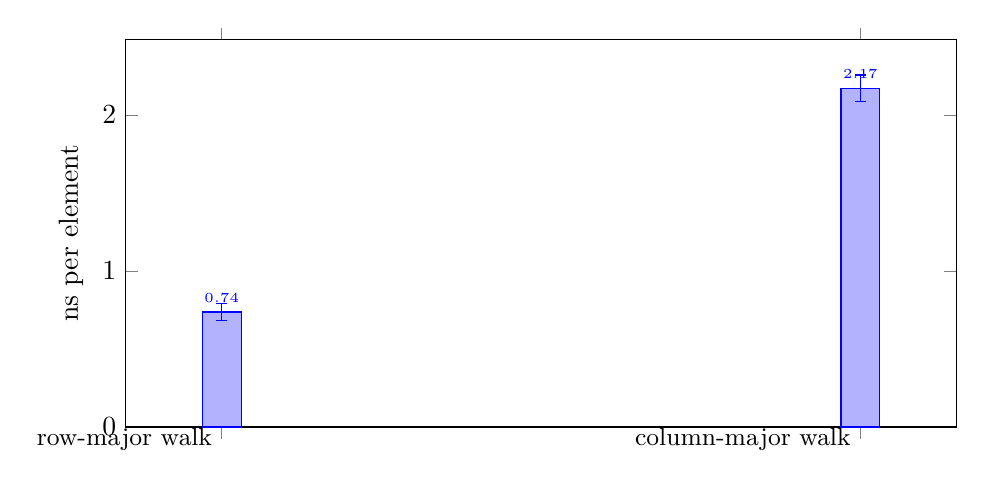
\begin{tikzpicture}
\begin{axis}[ybar, width=\textwidth, height=6.5cm, bar width=14pt, ymin=0, symbolic x coords={row-major walk,column-major walk}, xtick=data, x tick label style={rotate=0, anchor=east, font=\small}, ylabel={ns per element}, enlarge x limits=0.15, legend style={font=\small, at={(0.98,0.98)}, anchor=north east}, nodes near coords, nodes near coords style={font=\tiny}, every node near coord/.append style={/pgf/number format/.cd, fixed, precision=2}]
\addplot+[error bars/.cd, y dir=both, y explicit] coordinates {(row-major walk,0.7372) +- (0,0.0562) (column-major walk,2.1692) +- (0,0.0863)};
\end{axis}
\end{tikzpicture}